\documentclass[]{article}

\usepackage[utf8]{inputenc}
\usepackage[english,serbian]{babel}
\usepackage[margin=0.7in]{geometry}
\usepackage{url}
\usepackage{float}
\usepackage[graphicx]{realboxes}
\usepackage{listings}
\usepackage{textcomp}
\usepackage{xcolor}
\usepackage{adjustbox}
\lstset {
    language=HTML,
    frame=none,
    %xleftmargin=-.25in,
    %xrightmargin=.25in
    framesep=10pt,
    tabsize=4,
    showstringspaces=false,
    upquote=true,
    commentstyle=\color{black},
    keywordstyle=\color{black},
    stringstyle=\color{black},
    basicstyle=\small\ttfamily,
    emph={int,char,double,float,unsigned,void,bool},
    emphstyle={\color{black}},
    escapechar=\&,
    classoffset=1,
    morekeywords={>,<,.,;,,,-,!,=,~},
    keywordstyle=\color{black},
    classoffset=0,
    breaklines=true
}
\pagenumbering{gobble}

\title{Ra\v{c}unarske mre\v{z}e 2019, Ispit - Januar 2, 4I}
\author{}
\date{30.01.2019.}

\begin{document}
\maketitle

\begin{enumerate}
  \item Sockets and Channels \textbf{(15p)}
  \begin{itemize}
    \item Napraviti Java aplikaciju koja ima ulogu klijenta. Povezati se na lokalni server na portu 12345 koriste\'c{}i Java Sockets API i u beskona\v{c}noj petlji ispisivati brojeve koje server \v{s}alje. Kada server prekine vezu, klijent se zaustavlja. \hfill (4p)
    \item Napraviti Java aplikaciju koja ima ulogu servera. Pokrenuti \textbf{neblokiraju\'c{}i} lokalni server na portu 12345 koriste\'c{}ci Java Channels API. Server svim klijentima \v{s}alje nasumi\v{c}no izabrani ceo broj. Klijent ispisuje dobijeni broj na standardni izlaz. \hfill (5p)
    \item Omogu\'c{}iti da server svakom klijentu po\v{s}alje ta\v{c}no pet brojeva u intervalima od pet sekundi između svakog slanja. \hfill (5p)
    \item Postarati se da su svi resursi ispravno zatvoreni u slu\v{c}aju izuzetka. \hfill (1p)
  \end{itemize}

  \item Swing \textbf{(15p)}
  Napraviti Java Swing aplikaciju koja ima ulogu jednostavnog Outliner-a. Izgled aplikacije je dat na slici ispod. HTML fajlovi su na slede\'c{}oj strani.
  \begin{itemize}
    \item Napraviti prozor i u njega dodati skrolabilnu komponentu za prikaz HTML sadr\v{z}aja. \hfill (2p)
    \item Dodati oblast za unos URL-a koji vodi do HTML fajla na lokalnom fajlsistemu. Dodati dugme \texttt{Prika\v{z}i} koje prikazuje sadr\v{z}aj tog HTML fajla u komponenti za prikaz. \hfill (2p)
    \item Ispo\v{s}tovati izgled aplikacije (ne me\v{s}ati redosled komponenti i postarati se da su odnosi u veli\v{c}ini kao na slici). \hfill (2p)
    \item Omogu\'c{}iti da se prozor mo\v{z}e pro\v{s}iriti i smanjiti a da se raspored i razmera komponenti ne promeni. \hfill (3p)
    \item Dodati dugme \texttt{Sadr\v{z}aj} \v{c}iji je efekat da kreira HTML listu naslova iz HTML sadr\v{z}aja komponente za prikaz. Uvu\'c{}i svaki naslov onoliko tab karaktera koliki je njegov nivo (npr. \texttt{<h3>} naslov se uvla\v{c}i 3 puta). Prikazati kreirani HTML u komponenti za prikaz. \hfill (6p)
  \end{itemize}

  \begin{figure}[H]
    \centering
    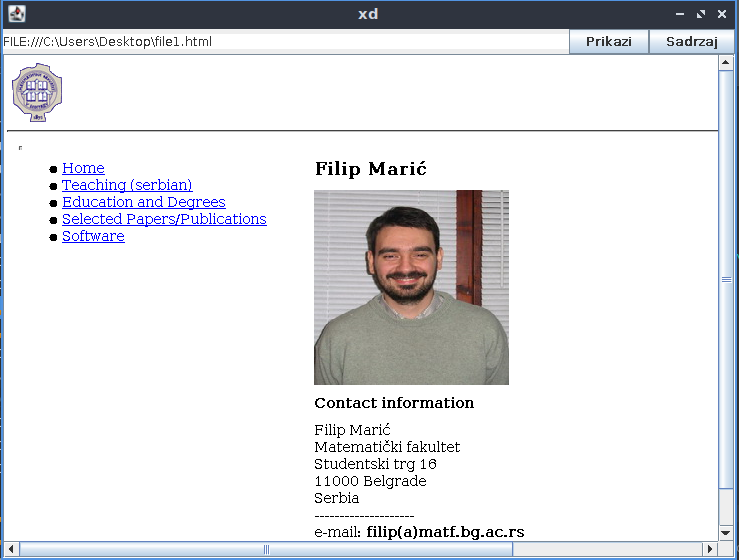
\includegraphics[scale=0.6]{fig2.PNG}
    \label{fig2}
  \end{figure}

\end{enumerate}

\newpage

HTML test fajlovi za zadatak 2:

\begin{itemize}
  \item 1.html
    \begin{lstlisting}
      <!DOCTYPE html>
        <html>
          <body>
            <h1>1.HTML 1</h1>
            <h2>1.HTML 2</h1>
            
            <p>My paragraph.</p>

            <h3>1.HTML 3</h1>
            <h4>1.HTML 4</h1>
            <h5>1.HTML 5</h1>
            <h6>1.HTML 6</h1>

            Test
          </body>
        </html>
    \end{lstlisting}
  \item 2.html
    \begin{lstlisting}
      <!DOCTYPE html>
        <html>
          <body>
            <h1>1.HTML 1</h1>
            <h2>1.HTML 2</h1>
            
            <p>My paragraph.</p>

            <h3>1.HTML 3</h1>

            Test

            <h1>1.HTML 1</h1>
          </body>
        </html>
    \end{lstlisting}
  \item 3.html
     \begin{lstlisting}
      <!DOCTYPE html>
        <html>
          <body>
            Test
            <h2>1.HTML 2</h1>
            <h4>1.HTML 4</h1>
            
            <p>My paragraph.</p>

            <h3>1.HTML 3</h1>

            Test

            <h1>1.HTML 1</h1>
          </body>
        </html>
    \end{lstlisting}
\end{itemize}


\end{document}
